\documentclass[10pt]{article}
\usepackage[utf8]{inputenc}
\usepackage[T1]{fontenc}
\usepackage{amsmath}
\usepackage{amsfonts}
\usepackage{amssymb}
\usepackage[version=4]{mhchem}
\usepackage{stmaryrd}
\usepackage{graphicx}
\usepackage[export]{adjustbox}
\graphicspath{ {./images/} }

\title{SOLUTIONS FOR EXTRA ADMISSIONS TEST IN MATHEMATICS, COMPUTER SCIENCE AND JOINT SCHOOLS DECEMBER 2022 }

\author{}
\date{}


\begin{document}
\maketitle
A Note that the probability that the coin does not land on heads is $1-\cos ^{2} \alpha=\sin ^{2} \alpha$. The probability of exactly two heads is $\left(\begin{array}{l}3 \\ 2\end{array}\right) \cos ^{4} \alpha \sin ^{2} \alpha$ and the probability of exactly three heads is $\left(\begin{array}{l}3 \\ 1\end{array}\right) \cos ^{6} \alpha$. Simplifying gives

$$
3 \cos ^{4} \alpha \sin ^{2} \alpha+\cos ^{6} \alpha=3\left(1-\sin ^{2} \alpha\right)^{2} \sin ^{2} \alpha+\left(1-\sin ^{2} \alpha\right)^{3}=1-3 \sin ^{4} \alpha+2 \sin ^{6} \alpha
$$

The answer is (d)

B If we write $u=e^{-x / 2}$ then the given expression is $u-u^{2}$. This quadratic has roots at 0 and 1 , and is positive in between. Now as $x$ varies from 0 to $\infty, u$ will decay exponentially from 1 to 0 . Along the way, $u-u^{2}$ will start at 0 , then vary through positive numbers, first increasing for $u>1 / 2$ then decreasing for $u<1 / 2$ and eventually tending towards 0 .

The answer is (a)

C The left-hand side factorises to give

$$
(x-1)(x-2)<\frac{(x-1)}{x}
$$

When are the two sides equal? That happens when $x=1$ or when $x(x-2)=1$, that is when $x=1 \pm \sqrt{2}$. Note that one of these roots is negative and the other is positive.

That helps us to draw a graph (it's perhaps useful to note that the right-hand side is $1-1 / x$ ).

\begin{center}
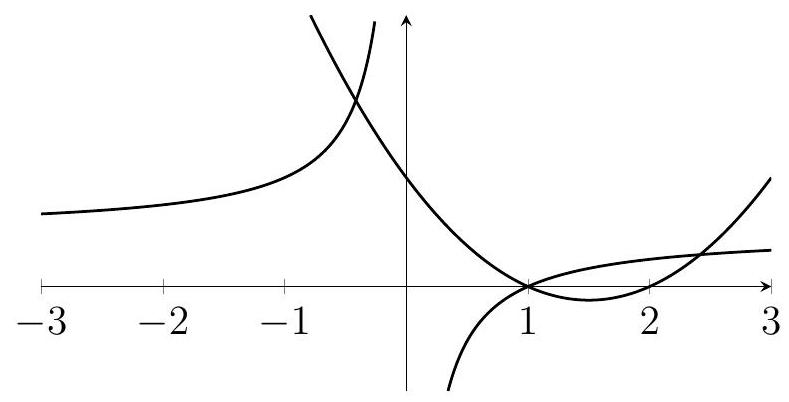
\includegraphics[max width=\textwidth]{2024_03_31_937c7aabca741f5fb902g-1(1)}
\end{center}

From the graph, we see that the quadratic is below the reciprocal graph for $1-\sqrt{<}<0$ and for $1<x<1+\sqrt{2}$.

The answer is (b)

D The first inequality describes a region between two concentric circles. The second inequality is true if either (case 1) $x \geq 0$ and $-x \leq \sqrt{3} y \leq x$, or (case 2) $x \leq 0$ and $x \leq \sqrt{3} y \leq-x$.

\begin{center}
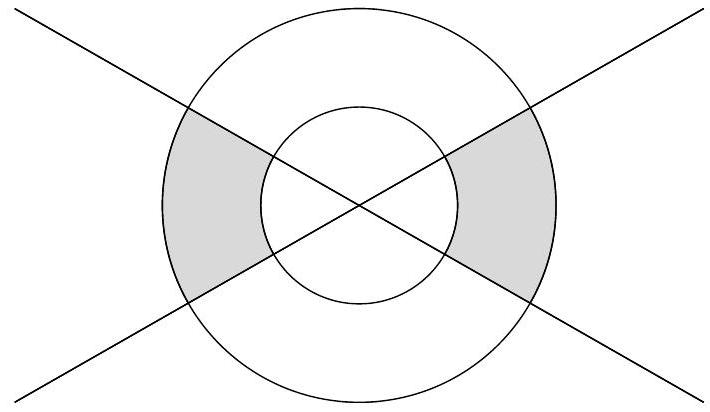
\includegraphics[max width=\textwidth]{2024_03_31_937c7aabca741f5fb902g-1}
\end{center}

The intersection points between the inner circle and those lines are $(\sqrt{3} / 2,1 / 2)$ and reflections, so the acute angle subtended at the origin by the two lines is $60^{\circ}$. We would therefore like one-third of the area between the two circles, which is $\frac{1}{3} \pi\left(2^{2}-1^{2}\right)=\pi$.

The answer is (b)

$\mathbf{E}$ The centre of the circle is $\left(\frac{p}{2}, \frac{q+1}{2}\right)$ and the radius is $\sqrt{\frac{p^{2}}{4}+\frac{(q-1)^{2}}{4}}$, so the equation of the circle is

$$
\left(x-\frac{p}{2}\right)^{2}+\left(y-\frac{q+1}{2}\right)^{2}=\frac{p^{2}}{4}+\frac{(q-1)^{2}}{4}
$$

On the line $y=0$, this a quadratic for $x$. We can set the discriminant equal to zero for a repeated solution. The quadratic is $x^{2}-p x+q=0$ and the discriminant is $p^{2}-4 q$.

\section*{The answer is (c)}
F We need $-1<1+x-x^{2}<1$. Let's find the points where $1+x-x^{2}=1$ (that's 0 and 1 ) and find the points where $1+x-x^{2}=-1$ (that's -1 and 2 ). Consider the graph.

\begin{center}
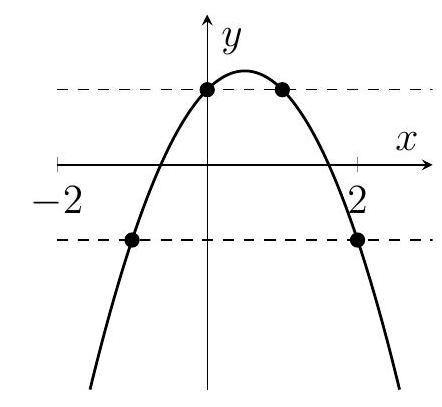
\includegraphics[max width=\textwidth]{2024_03_31_937c7aabca741f5fb902g-2}
\end{center}

We need either $-1<x<0$ or $1<x<2$.

The answer is (c)

G All of the options are of the form $y=k f(x)$ with $k$ constant so let's try that in the equation. We get $k \frac{\mathrm{d} f(x)}{\mathrm{d} x}$ on the left and $2(k f(x))^{1 / 4}$ on the right. Now $\frac{\mathrm{d} f(x)}{\mathrm{d} x}=(f(x))^{1 / 4}$ so we just need $k=2 k^{1 / 4}$. We can rearrange this to get $k=2^{4 / 3}$.

The answer is (c)

H Clearly $f$ is always a positive whole integer from the recursion relations.

First find $n$ with $f(n)=1$. Because $f(2 n)=f(n)$ and $f(1)=1$, it must be the case that for all powers of $2, f(n)=1$. On the other hand, $f(2 n+1)=f(n)+f(n+1)$ is definitely at least two, so $f(n)$ is only equal to 1 on the powers of 2 .

Next consider values of $n$ for which $f(n)=2$. The first equation shows us that if we have $n$ even and $f(n)=2$ then $f(n / 2)=2$. Let's suppose instead that $n$ is odd and write $n=2 m+1$. Then we would have $f(n)=f(m)+f(m+1)$. The only way for this to be 2 is if the right-hand side is $1+1$, which only happens if both the consecutive numbers $m, m+1$ are powers of 2 , which only happens for 1,2 . Check that $f(3)=f(1)+f(2)=2$. So the points where $f(n)=2$ are precisely those where $n$ is three times a power of 2 (they're of the form $3 \times 2^{k}$ ).

Now finally consider values of $n$ for which $f(n)=3$. The first equation again tells us that we can multiply any such $n$ by 2 . Let's look for odd solutions. They must come from $1+2$ on the right-hand side of the second equation, which only happens if a power of $2\left(2^{l}\right.$ say) is one more or one less than a number of the form $3 \times 2^{k}$. That's a bit unusual though, because both $2^{l}$\\
and $3 \times 2^{k}$ are even, unless one of the powers of 2 is equal to 1 . So those consecutive numbers must be either 2 and 3 or they could be 3 and 4 . This gives $f(5)=3$ and $f(7)=3$, but that's it for odd numbers. The solutions to $f(n)=3$ are therefore $5 \times 2^{k}$ or $7 \times 2^{k}$. None of these are multiples of 35 .

\section*{The answer is (a)}
I Take two to the power of each side for $x=(x+a) 2^{b}$

The right-hand side is a line with gradient $2^{b}$ and $y$-intercept $a 2^{b}$. We're looking for positive solutions, and there are two ways this could happen; either $a 2^{b}$ is larger than zero, but the line grows slower than $x$, or $a 2^{b}$ is negative but the line grows faster than $x$. This corresponds to (in the first case) $a>0$ and $b<0$, or (in the second case) $a<0$ and $b>0$. Either way, $a b<0$. There's only one intersection between two straight lines, if any.

The answer is (c)

J Consider adding together these integrals to get

$$
\int_{1}^{2} \frac{x^{2}+x^{-2}}{1+x^{4}} \mathrm{~d} x
$$

Now note that the numerator is $x^{-2}$ multiplied by the denominator, so this simplifies to

$$
\int_{1}^{2} x^{-2} \mathrm{~d} x=\left[-x^{-1}\right]_{1}^{2}=\frac{1}{2}
$$

The integral we're asked for is therefore $\frac{1}{2}-A$.

The answer is (e)


\end{document}